% !TeX root = ../../main.tex
\section{Process design data sheets}

\subsection{Key reactor}
\begin{table}[H]
    \centering
    \begin{tabular}{@{}l|l@{}}
    \toprule
      \textbf{Equipment label}  & R101\\
       \textbf{Equipment type}  & Heat Exchanger Reactor (HEX) \\
       \textbf{Material of construction} & Stainless steel 304L \\
       \bottomrule
    \end{tabular}
\end{table}


\begin{figure}[H]
    \centering
    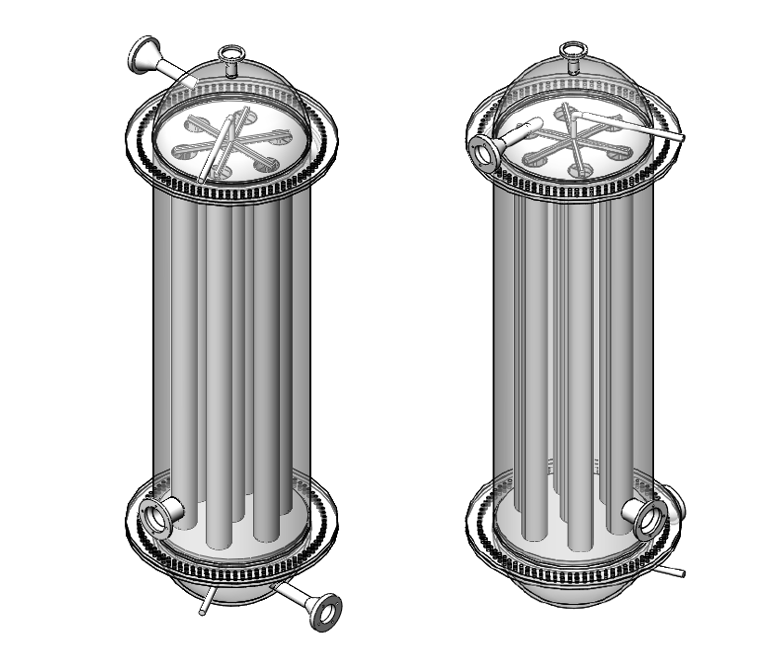
\includegraphics[width=0.7\linewidth]{chapters/2-reaction/figures/FYD reactor poster boy both.PNG}
    \caption{3D Reactor model}
\end{figure}

\begin{table}[H]
\centering
\begin{tabular}{@{}l|l|l@{}}
\toprule
\textbf{Specification}                    & \textbf{Value} & \textbf{Units} \\ \midrule
Max Temperature                           & 90             & °C             \\ \midrule
Cooling duty                              & 63.4         & kW                \\ \midrule
Inlet   pressure, P1                      & 130        & kPa            \\ \midrule
Outlet   pressure, P2                     & 100            & kPa            \\ \midrule
Design   pressure                       & 144        & kPa            \\ \midrule
Maximum   allowable accumulated  pressure & 174        & kPa            \\ \midrule
Reactor length                            & 4.3          & m               \\ \midrule
Reactor tube diameter                            & 0.23          & m               \\ \midrule
Reactant flowrate                         & 11.354         & mm$^2$            \\ \midrule
Primary cooling water flowrate            & 2.3           & kg/s             \\ \midrule
Secondary cooling water flowrate          & 2.1         & kg/s            \\ \midrule
Shell and end thickness                   & 5         & mm            \\ \bottomrule
\end{tabular}
\end{table}
\newpage

\subsection{Key separator}

\begin{table}[H]
    \centering
    \begin{tabular}{@{}l|l@{}}
    \toprule
      \textbf{Equipment label}  & S104\\
       \textbf{Equipment type}  & Melt crystalliser \\
       \textbf{Material of construction} & Stainless steel 304L-S71 \\
       \bottomrule
    \end{tabular}
\end{table}


\begin{figure}[H]
    \centering
    \includesvg[inkscapelatex=false,scale=0.5]{chapters/3-separation/figures/Crystalliser_schematic.svg}
    \caption{3D schematics for the designed crystalliser vessel: (i) perspective view; (ii) section view.}
    \label{fig:schematic crystalliser process design data sheet}
\end{figure}

\begin{table}[H]
\centering
\begin{tabular}{@{}l|l|l@{}}
\toprule
\textbf{Specification}                  & \textbf{Value} & \textbf{Units}    \\ \midrule
Inlet temperature                       & 331             & K                \\ \midrule
Operating temperature                   & 280             & K                \\ \midrule
Total mass flowrate                     & 1246.28         & ton/yr             \\ \midrule
Operating pressure                      & 1               & atm               \\ \midrule
Height                                  & 0.9864          & m                 \\ \midrule
Diameter                                & 0.4932          & m                 \\ \midrule
Cooling coil pitch length               & 0.072           & m                 \\ \midrule
Cooling coil outer diameter             & 0.062           & m                  \\ \bottomrule
\end{tabular}
\end{table}

\newpage
\subsection{Heat exchanger}

\begin{table}[H]
    \centering
    \begin{tabular}{@{}l|l@{}}
    \toprule
    \textbf{Pocess Equipment}      & Heat Exchanger      \\
    \textbf{Equipment Label}       & S201 condenser      \\
    \textbf{Equipment Model}       & Plate   \& Frame    \\
    \textbf{Construction Material} & 316 Stainless Steel \\ \bottomrule
    \end{tabular}
\end{table}

\begin{figure}[H]
    \centering
    \begin{subfigure}{0.49\linewidth}
        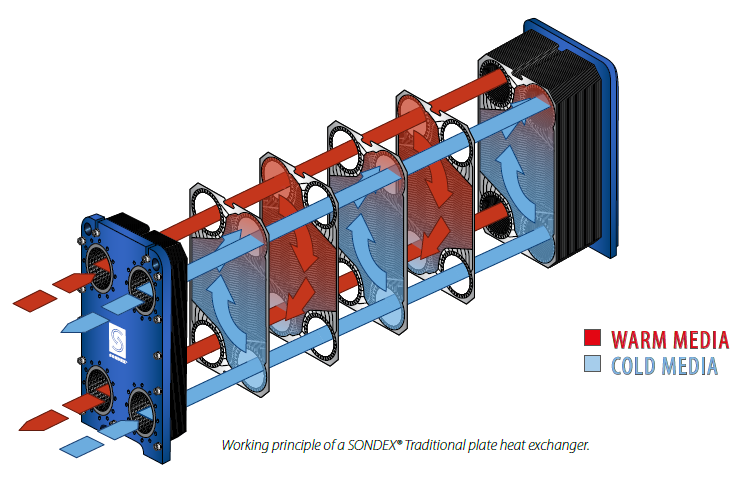
\includegraphics[width=\linewidth]{chapters/Z-support/figures/hex_schematic.png}
        \caption{PHEX Schematic []}
    \end{subfigure}
    \begin{subfigure}{0.49\linewidth}
        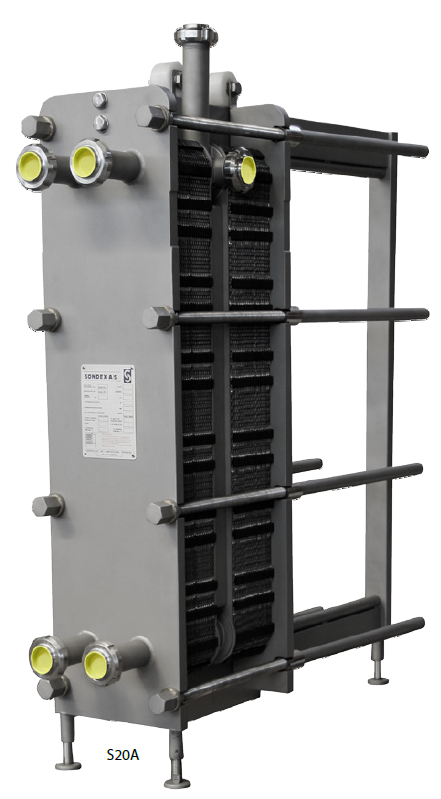
\includegraphics[width=0.49\linewidth]{chapters/Z-support/figures/hex_diagram.png}
        \caption{PHEX Image []}
    \end{subfigure}
\end{figure}

\begin{table}[H]
\centering
\begin{tabular}{@{}l|l|l@{}}
\toprule
\textbf{Specification}           & \textbf{Value}                       & \textbf{Units} \\ \midrule
Total heat   exchange area       & 5.83                                 & m2             \\ \midrule
Heat exchange   area per plate   & 0.10                                 & m2             \\ \midrule
Number of   plates               & 59                                   &                \\ \midrule
Plate   dimensions (HxW)         & \multicolumn{1}{r|}{394*126}         & mm             \\ \midrule
Cooling duty                     & -335                                 & kW             \\ \midrule
Flow type                        & \multicolumn{1}{r|}{Counter-current} &                \\ \midrule
Feed flowrate                    & 226                                  & kg/h           \\ \midrule
Cooling water   flowrate         & 146                                  & kg/h           \\ \midrule
Hot stream   inlet temperature   & 67                                   & °C             \\ \midrule
Hot stream   outlet temperature  & 67                                   & °C             \\ \midrule
Cold stream   inlet temperature  & 16                                   & °C             \\ \midrule
Cold stream   outlet temperature & 57                                   & °C             \\ \midrule
LMTD                             & 57                                   & °C             \\ \midrule
Heat transfer   coefficient      & 1007                                 & W/(m2.K)       \\ \bottomrule
\end{tabular}
\end{table}


\newpage
\subsection{Safety relief valve}

\begin{table}[H]
    \centering
    \begin{tabular}{@{}l|l@{}}
    \toprule
      \textbf{Equipment label}  & PRV-1 on R201\\
       \textbf{Equipment type}  & Safety pressure relief valve \\
       \textbf{Material of construction} & Stainless steel 316 \\
       \bottomrule
    \end{tabular}
\end{table}


\begin{figure}[H]
    \centering
    \begin{subfigure}{0.49\linewidth}
        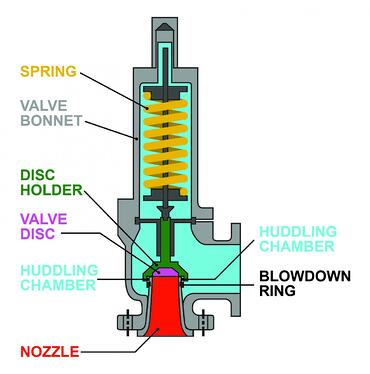
\includegraphics[width=\linewidth]{chapters/Z-support/figures/PSV_Diagram.jpg}
        \caption{PRV Schematic \cite{smith_spring_nodate}}
    \end{subfigure}
    \begin{subfigure}{0.49\linewidth}
        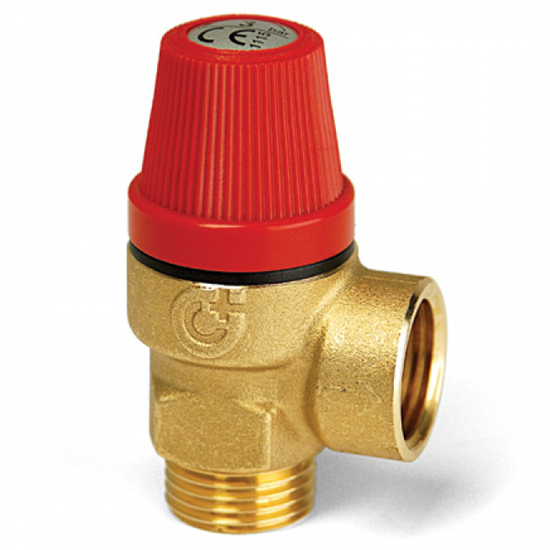
\includegraphics[width=\linewidth]{chapters/Z-support/figures/product_a_l_altecnic-caleffi-safety-relief-valve-1-2-6-bar-312460-small.jpg}
        \caption{PRV Image \cite{unvented_components_europe_caleffi_nodate}}
    \end{subfigure}
\end{figure}

\begin{table}[H]
\centering
\begin{tabular}{@{}l|l|l@{}}
\toprule
\textbf{Specification}                    & \textbf{Value} & \textbf{Units} \\ \midrule
Temperature                               & 60             & °C             \\ \midrule
Max discharge   flowrate                  & 11.779         & kg/hr          \\ \midrule
Ratio of   specific heats (Cp/Cv)  \cite{api_standard_520_sizing_2013}      & 1.41           &                \\ \midrule
Inlet   pressure, P1                      & 506.625        & kPa            \\ \midrule
Outlet   pressure, P2                     & 101            & kPa            \\ \midrule
Critical   pressure                       & 266.790        & kPa            \\ \midrule
Maximum   allowable accumulated  pressure & 596.544        & kPa            \\ \midrule
Efficient   discharge coefficient  []        & 0.975          &                \\ \midrule
Required   discharge area                 & 11.354         & mm$^2$            \\ \midrule
Nominal nozzle   size                     & 3.80           & mm             \\ \bottomrule
\end{tabular}
\end{table}

\newpage
\subsection{Control valve}


\begin{table}[H]
    \centering
    \begin{tabular}{@{}l|l@{}}
    \toprule
      \textbf{Equipment label}  & FCV-203 on 2-06\\
       \textbf{Equipment type}  & Type 3323 - Bürkert diaphragm valve \cite{noauthor_type_nodate}\\
       \textbf{Material of construction} & Stainless steel 316 \\
       \bottomrule
    \end{tabular}
\end{table}

\begin{figure}[H]
    \centering
    \begin{subfigure}{0.49\linewidth}
        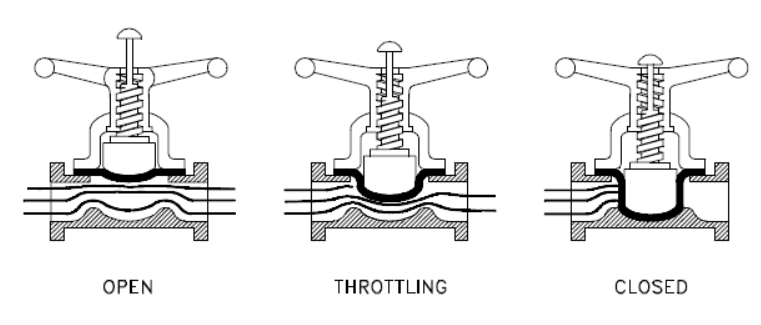
\includegraphics[width=\linewidth]{chapters/Z-support/figures/fcv_diagram.PNG}
        \caption{FCV Schematic \cite{noauthor_type_nodate}}
    \end{subfigure}
    \begin{subfigure}{0.49\linewidth}
        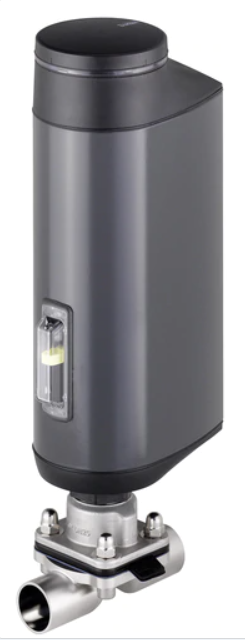
\includegraphics[width=0.49\linewidth]{chapters/Z-support/figures/fcv.PNG}
        \caption{FCV Image \cite{noauthor_diaphragm_nodate}}
    \end{subfigure}
\end{figure}

\begin{table}[H]
\centering
\begin{tabular}{@{}l|l|l@{}}
\toprule
\textbf{Specification}                    & \textbf{Value} & \textbf{Units} \\ \midrule
Maximum ambient temperature                               & 50             & °C             \\ \midrule
Maximum operating pressure                  & 1000        & kPa        \\ \midrule
Normal operating pressure       & 101         &     kPa           \\ \midrule
Feed normal flowrate                      & 0.67      & m$^3$/h           \\ \midrule
Diaphragm material   \cite{noauthor_diaphragm_nodate}                & Viton           &            \\ \midrule
External diameter of pipe                      & 21.3     & mm            \\ \midrule
Diaphragm size & 15     & mm           \\ \midrule
Port connection       & 15         & mm                \\ \bottomrule
\end{tabular}
\end{table}

\newpage
\subsection{Pump}

\begin{table}[H]
    \centering
    \begin{tabular}{@{}l|l@{}}
    \toprule
      \textbf{Equipment label}  & P201a/b \\
       \textbf{Equipment type}  & tapflo CTI AA Centrifugal Pump \cite{tapflo_cti_nodate}\\
       \textbf{Material of construction} & Stainless steel 316 \\
       \bottomrule
    \end{tabular}
\end{table}

\begin{figure}[H]
    \centering
    \begin{subfigure}{0.49\linewidth}
        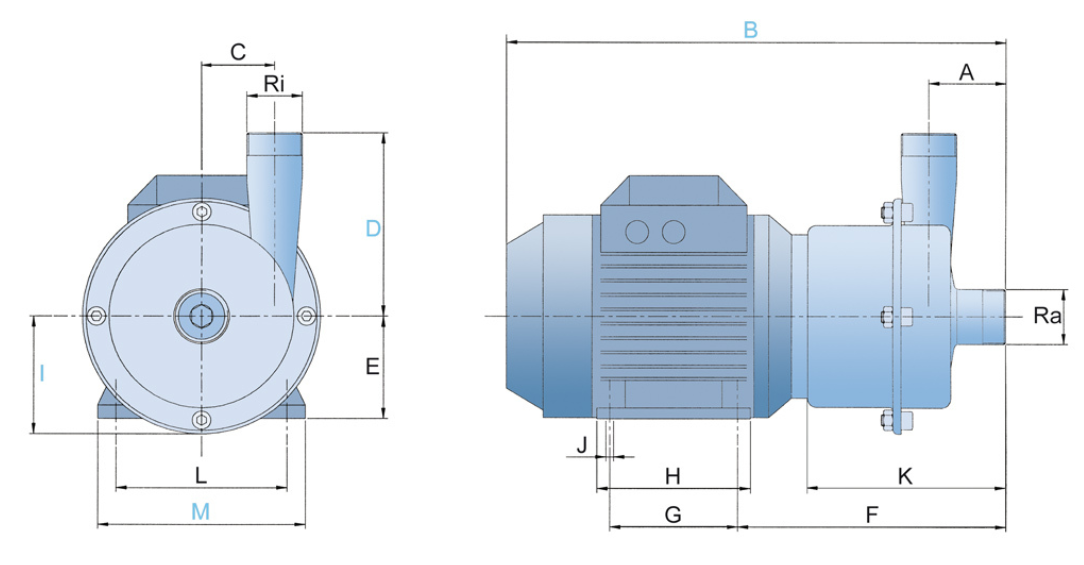
\includegraphics[width=\linewidth]{chapters/Z-support/figures/pump_schematic.PNG}
        \caption{Pump Schematic \cite{tapflo_cti_nodate}}
    \end{subfigure}
    \begin{subfigure}{0.49\linewidth}
        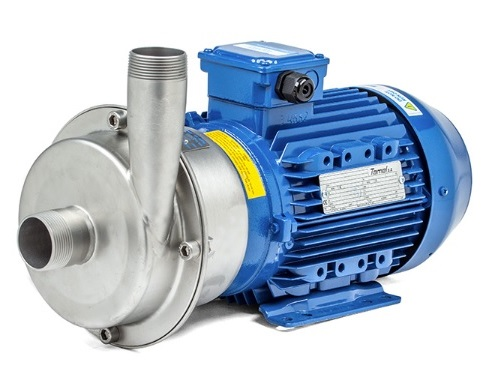
\includegraphics[width=\linewidth]{chapters/Z-support/figures/pump_image.jpg}
        \caption{Pump Image \cite{tapflo_cti_nodate}}
    \end{subfigure}
\end{figure}

\begin{table}[H]
\centering
\begin{tabular}{@{}l|l|l@{}}
\toprule
\textbf{Specification}                    & \textbf{Value} & \textbf{Units} \\ \midrule
Discharge volume                              & 0.65            & m$^3$/h            \\ \midrule
Maximum capacity                  & 12       &  m$^3$/h       \\ \midrule
Maximum discharge pressure       & 10         &     bar           \\ \midrule
Maximum temperature                  & 90     & °C         \\ \midrule
Pump efficiency \cite{pumps_and_systems_magazine_pump_2012}               & 65\%         &            \\ \midrule
Maximum pumping power                     & 0.55     & kW           \\ \bottomrule
\end{tabular}
\end{table}

\newpage
\subsection{Storage vessel}
\begin{table}[H]
    \centering
    \begin{tabular}{@{}l|l@{}}
    \toprule
      \textbf{Equipment label}  & SV101\\
       \textbf{Equipment type}  & Storage Vessel \\
       \textbf{Material of construction} & Stainless steel 316 \\
       \bottomrule
    \end{tabular}
\end{table}

\begin{figure}[H]
    \centering
    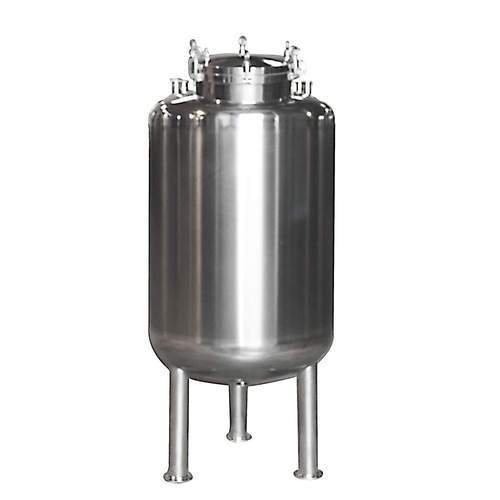
\includegraphics[width=\linewidth]{chapters/Z-support/figures/stainless-steel-storage-tank-500x500.jpg}
    \caption{Storage tank []}
\end{figure}

\begin{table}[H]
\centering
\begin{tabular}{@{}l|l|l@{}}
\toprule
\textbf{Specification}                    & \textbf{Value} & \textbf{Units} \\ \midrule
Volume                              & 1            & L            \\ \midrule
Temperature                     & 120     & C           \\ \bottomrule
\end{tabular}
\end{table}




\newpage
\subsection{Flare stack}

\begin{figure}[H]
    \centering
    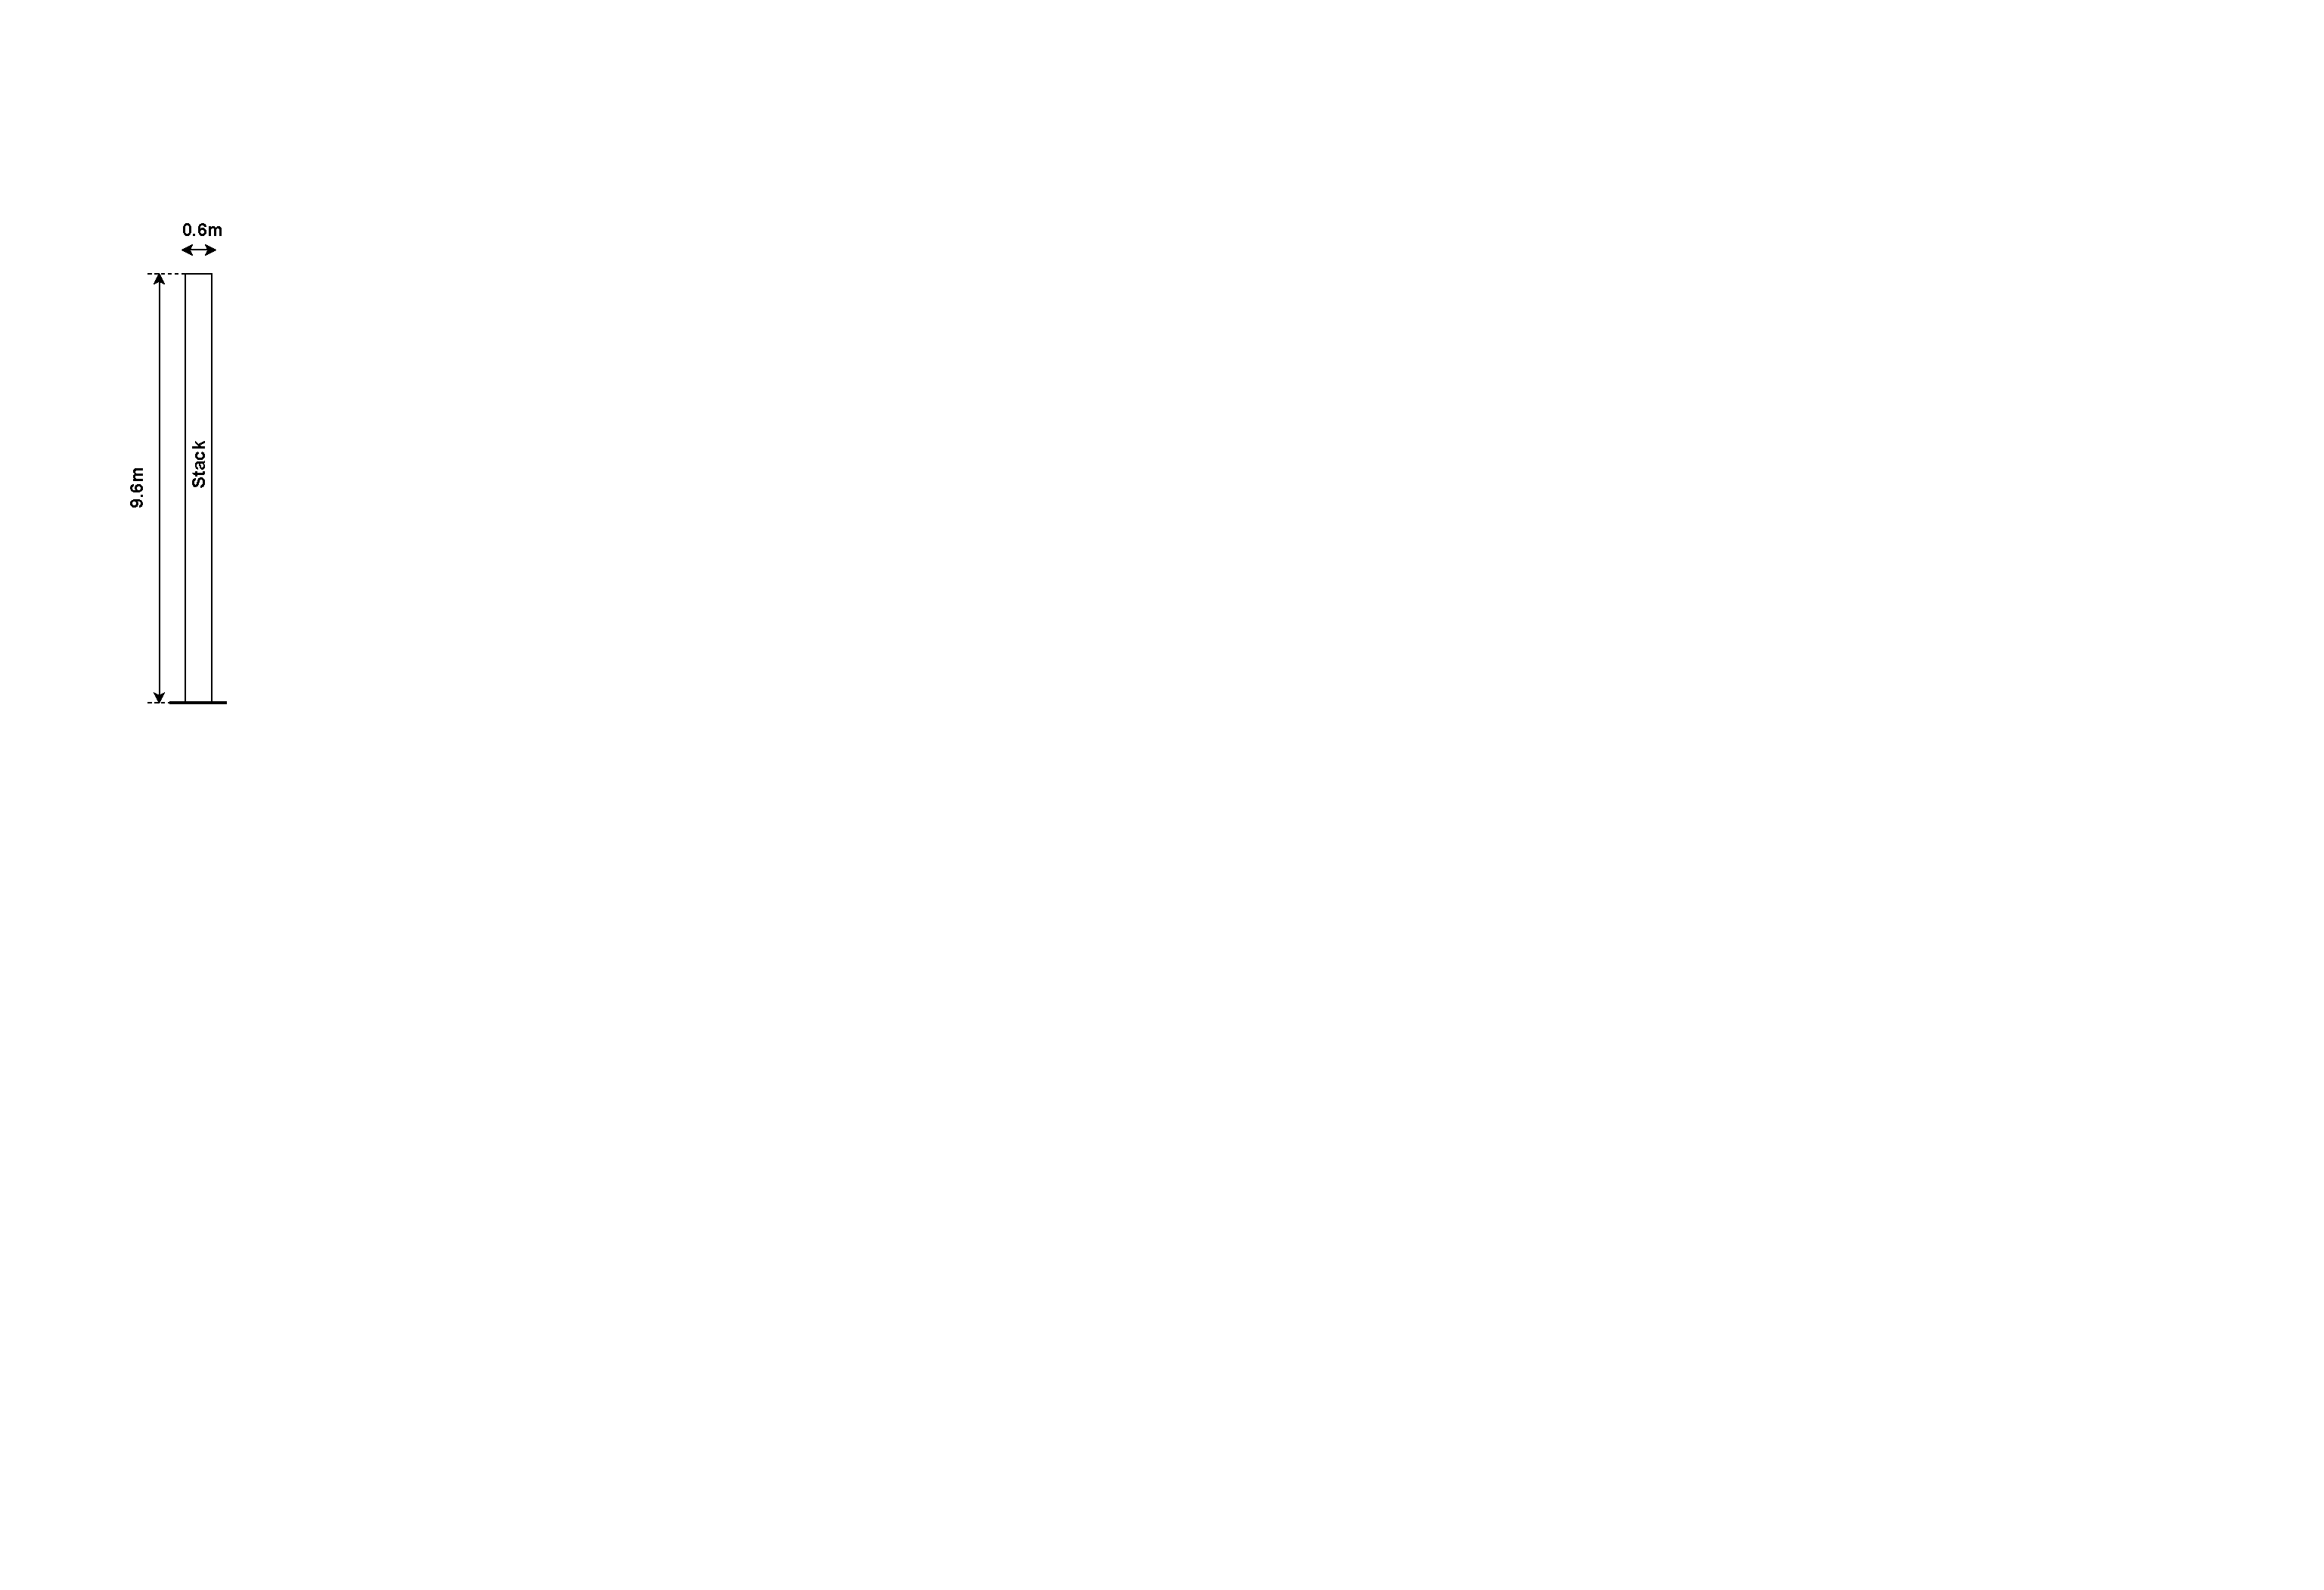
\includegraphics[width=\linewidth]{chapters/Z-support/figures/Flue gas stack.pdf}
    \caption{Flue gas stack}
\end{figure}

\begin{table}[H]
\caption{Flue gas stack }
\label{tab:fluestack}
\begin{tabular}{lc}
\textbf{Process Equipment}                    & Flue gas stack (for waste treatment emissions) \\
\textbf{Stack Height (m)}                     & 9.6                                            \\
\textbf{Internal Stack Diameter (m)}          & 0.6                                            \\
\textbf{Average wind speed (m/s)}             & 3.2                                            \\
\textbf{Gas outlet velocity (m/s)}            & 0.02                                            \\
\textbf{Average atmospheric temperature (°C)} & 21                                             \\
\textbf{Average flue gas temperature (°C)}    & 140                                            \\
\textbf{Material used}                        & Stainless steel 316                           
\end{tabular}
\end{table}


\newpage
\subsection{Hydraulic wash column}

\begin{table}[H]
    \centering
    \begin{tabular}{@{}l|l@{}}
    \toprule
      \textbf{Equipment label}  & S106\\
       \textbf{Equipment type}  & Hydraulic wash column \\
       \textbf{Material of construction} & Stainless steel 304L-S71 \\
       \bottomrule
    \end{tabular}
\end{table}


\begin{figure}[H]
    \centering
    \includesvg[inkscapelatex=false,scale=0.5]{chapters/3-separation/figures/Wash_column_schematic_executive.svg}
    \caption{3D schematics for the designed crystalliser vessel: (i) perspective view; (ii) right-side section; (iii) front section}
    \label{fig:schematic wash column process design data sheet}
\end{figure}

\begin{table}[H]
\centering
\begin{tabular}{@{}l|l|l@{}}
\toprule
\textbf{Specification}                  & \textbf{Value}  & \textbf{Units}    \\ \midrule
Inlet temperature                       & 280             & K                \\ \midrule
Bottom temperature                      & 324             & K                \\ \midrule
Total inlet mass flowrate               & 1246.28         & ton/yr             \\ \midrule
Solid flowrate                          & 0.03161         & kg/s             \\ \midrule
Operating pressure                      & 1               & atm               \\ \midrule
Height                                  & 0.800           & m                 \\ \midrule
Diameter                                & 0.170           & m                 \\ \midrule
Filter tube length                      &  0.680          & m                 \\ \midrule
Filter tube diameter                    &  0.020          & m                  \\ \bottomrule
\end{tabular}
\end{table}
\newpage
\subsection{Refrigerator}

\begin{table}[H]
    \centering
    \begin{tabular}{@{}l|l@{}}
    \toprule
      \textbf{Equipment label}  & C102\\
       \textbf{Equipment type}  & Refrigerator \\
    \textbf{Manufacturer}  & Airedale \\
     \textbf{Product name}  & TurboChill FreeCool TCC11R04G-01 \\
          \textbf{Refrigerant}  & R1234ze \\
       \textbf{Material of construction} & Galvanised steel and aluminium \\
       \bottomrule
    \end{tabular}
\end{table}


\begin{figure}[H]
    \centering
    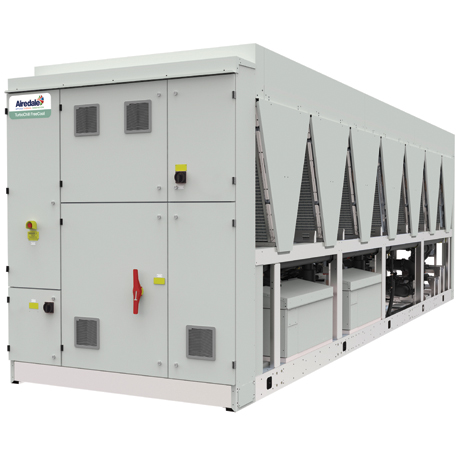
\includegraphics[scale=0.5]{chapters/3-separation/figures/Refrigerator.jpg}
    \caption{Image of an Airedale TurboChill$^{TM}$ FreeCool TCC11R04G-01 refrigerator}
    \label{fig:schematic refrigerator process design data sheet}
\end{figure}

\begin{table}[H]
\centering
\begin{tabular}{@{}l|l|l@{}}
\toprule
\textbf{Specification}                  & \textbf{Value} & \textbf{Units}    \\ \midrule
Cooling duty                            & 180             & kW                \\ \midrule
Power requirement                       & 52             & kW                \\ \midrule
Refrigerant charge                      & 110            & kg             \\ \midrule
Evaporator water flow rate              & 7.3            & L/s               \\ \midrule
Maximum airflow                         & 25.3           & m$^{3}$/s                 \\ \midrule
Dimensions                              & 2800 \times 2200 \times 2626           & mm$^{3}$   \\ \bottomrule
\end{tabular}
\end{table}